\documentclass[compsoc,draftclsnofoot,onecolumn,10pt]{IEEEtran}
\usepackage[utf8]{inputenc}
\usepackage{color}
\usepackage{url}

\usepackage{enumitem}

\usepackage[letterpaper, margin=.75in]{geometry}
\usepackage{hyperref}
\usepackage{listings}

\usepackage[dvipsnames]{xcolor}
\newcommand*{\SignatureAndDate}[1]{
    \par\noindent\makebox[2.5in]{\hrulefill} \hfill\makebox[2.0in]{\hrulefill}
    \newline\noindent\makebox[2.5in][l]{#1}  \hfill\makebox[2.0in][l]{Date}
}
\usepackage{etoolbox}
\patchcmd{\thebibliography}{\section*}{\subsection}{}{}
\patchcmd{\thebibliography}{\addcontentsline{toc}{section}{\refname}}{}{}{}

\usepackage{graphicx}
\usepackage{float}

\definecolor{dkgreen}{rgb}{0,0.6,0}
\definecolor{gray}{rgb}{0.5,0.5,0.5}
\definecolor{mauve}{rgb}{0.58,0,0.82}

\renewcommand{\lstlistingname}{Code Example} % a listing caption title.

\lstset{
	frame=single,
	language=C,
	columns=flexible,
	numbers=left,
	numbersep=5pt,
	numberstyle=\tiny\color{gray},
	keywordstyle=\color{blue},
	commentstyle=\color{dkgreen},
	stringstyle=\color{mauve},
	breaklines=true,
	breakatwhitespace=true,
	tabsize=4,
	captionpos=b
}

\def\name{Cierra Shawe, Daniel Stoyer, Tao Chen}

%% The following metadata will show up in the PDF properties
\hypersetup{
	colorlinks = false,
	urlcolor = black,
	pdfauthor = {\name},
	pdfkeywords = {ARC,Progress,Report, Winter,2017},
	pdftitle = {Arc Progress Report, Winter 2017},
	pdfsubject = {Progress Report for ARC},
	pdfpagemode = UseNone
}

\def\myversion{1.0 }
\date{}
%
%\usepackage{titlesec}
%
%\usepackage{hyperref}

\parindent = 0.0 in
\parskip = 0.1 in

\setcounter{secnumdepth}{5}

\begin{document}

\begin{titlepage}
\title{
Midterm Progress Report\\
\LARGE
ARC - Autonomous RC\\
Senior Capstone Project\\
Oregon State University\\
Winter 2017
}
\author{Tao Chen, Cierra Shawe, Daniel Stoyer}
\maketitle
\begin{center}
	Version 1.0\\
	\today
\end{center}

\thispagestyle{empty} % gets rid of the "0" page number.
	
\end{titlepage}

\tableofcontents

\newpage

\section{Project purpose and goals} 
% Breifly recaps project purpose and goals
The purpose of the Autonomous RC (ARC) project is to determine if it is possible
to build an autonomous RC vehicle using commodity components, meaning components
that are relatively inexpensive and can be bought at places like Radio
Shack\textsuperscript{\textregistered}, Best Buy\textsuperscript{\textregistered}, or on Amazon. \\
Our goal is to make an RC vehicle navigate autonomous to a given
waypoint/location, preferably at a high rate of speed and with obstacle avoidance. Stretch goals are to
make the vehicle drift around corners and parallel park.\\

%\[Be sure to add graphic back in before final render!!\]
\begin{figure}[H]
   	\includegraphics[width=\textwidth]{images/autorally_platform_header}
    \caption{Drifting example. Image from https://autorally.github.io/}
\end{figure}

While our main goal is to have a functioning autonomous RC vehicle we also hope
that we can produce instructions that RC enthusiasts can follow to produce a
functioning, consumer-grade autonomous RC vehicle of their own.

\section{Cierra}
	\subsection{Current Status}
		% what is the current status of your areas of focus?
		Over the past six weeks, my focus has been acquiring hardware, modifying and building hardware and components, and working on the vision system. 
		Currently, I have obtained all of the hardware we will need according to our design document minus the car. 
		In the beginning of the term I modeled a mount that is adjustable and meant to be used with the two USB cameras we were provided. 
		It is designed to be adjustable until we know how the cameras will need to be adjusted. 
		After having printed, acquired the baby screws required, and assembled the camera, I found the cords to be messy. 
		I fixed that with an expandable wiring sleeve that fits into the back of the camera case and expands in such a way that it doesn't slip out the back. 
		The next step was calibrating the cameras, which had a very steep learning curve due to learning the libraries for openCV, which is a cross-platform vision processing library. 
		As of now I am able to receive input from both cameras and create a disparity map. 
		The main problem is the updates slow and even after calibrating the cameras and the depth is often distorted from the cameras trying to auto-focus. 
		Hopefully, this week we will receive the Leddar M16, which is a Multi-element sensor module that uses 16 individual solid-state sensors to do time of flight sensing. 
		The M16 was designed for industrial applications and the company provides a "trial" kit which provides everything needed including the module, SDK, and C libraries for using the sensor.
		Due to the ability to detect multiple objects up to 150ft and providing a 45 degree view range, the M16 will probably end up replacing the stereo vision system, which isn't working as well as I would have hoped. 
		The RC will namely need to track objects in front of it, so the 45 degree field of view should be enough. 
		Using the M16 would also be able to allow us to switch to using a board such as the UPboard in place of the NUC, as it is only ever tracking 16 points at once. 
		This is significantly less complex than having to run complex algorithms for pixel matching and point cloud creation that we would need to do for stereo vision. 
		
		We were given a UM7, which didn't have any headers on it, which meant we had no way to communicate with the sensory. 
		I soldered on ends to the UM7, which was a challenge due to never having soldered and not understanding how wiring diagrams work.
		 Currently, using the software provided by RedShift Labs, I am able to visualize the data on a Windows computer. 
		This is rather cool, as once the major motion has gone away, if you place your finger on the sensor, the UM7 sensitive enough to notice a slight change in temperature and display your heart beat. 
		
		
				% Be sure to include descriptions of experimental design and use images, screenshots, code blocks
		
	\subsection{Left to do:}
		Once the Leddar unit arrives, this section could be vastly different. Most of the documentation for the unit is protected; however, it will be included when the testing package arrives. 
		Once we have the unit in hand, I will begin testing if it will be able to replace the stereo rig. 
		If the Leddar is able to preform to our needs, i.e. give fast enough readings at a wide enough range and we will need to see what libraries are available. 
		In order to test whether the M16 will work, I would like to take it outside, and see if it is able to detect things such as trees, walls, curbs, and rocks. 
			
		On top of that, as I oversee the hardware component protection of this project, I plan on creating a case for any component that is currently exposed. 
		As of now, that includes the Raspberry Pi 3 with the PXFmini shield, UM7, and a protective "roll" cage for the Intel Nuc, or possibly a smaller main computer if we are able to move away from the NUC, as the main challenge was being able to process vision. 
		We will also need to ensure that we are properly able to power all of our extra hardware, which currently will mean adding an extra LiPo battery.
		As a group, we still need to be able to fully control the servos and Electronic Speed Controller (ESC), and once we know what hardware we will finally use, I will turn our mock up into either an array of components mounted onto an acrylic/polycarbonate plate, or a complete box that all components can be contained within. 
		% What do you have left to do?
		\begin{itemize}
			\item Something to do...
		\end{itemize}
	\subsection{Challenges}
		
		\begin{tabular}{|p{0.3\linewidth}|p{0.3\linewidth}|}
			\hline
			\textbf{Problems} & \textbf{Solutions}\\
			\hline
			Problems that impeded progress. & Specific actions to resolve problems.\\
			\hline
						
		\end{tabular}
		
\section{Tao}
\subsection{Current Status}
My work was mostly on simulation of the platform on the computer. My strategies was to use as much AutoRally's code as possible. The AutoRally package contains a model description of the vehicle it uses. We are not using the same vehicle for our project. But it will be good enough for the simulation. When we get our hands on our vehicle, we can adjust some of the model parameters to best fit our vehicle. The AutoRally package also has a controller that is in Python to control the steering, which uses the Ackerman steering theory, and the forward/backward motion. \par     

As for right now, I still haven't written any code yet. I teared apart the AutoRally package and tried to understand it. I migrated a minimum amount of code to our own package such that the simulation would still run. That being said, when we are ready to build our platform and start implementation, we will use the current package as the foundation. The simulation of the platform will not drive itself yet. It has to be controlled by a Xbox controller (See figures below). \par 

\begin{figure}[H]
  \centering
  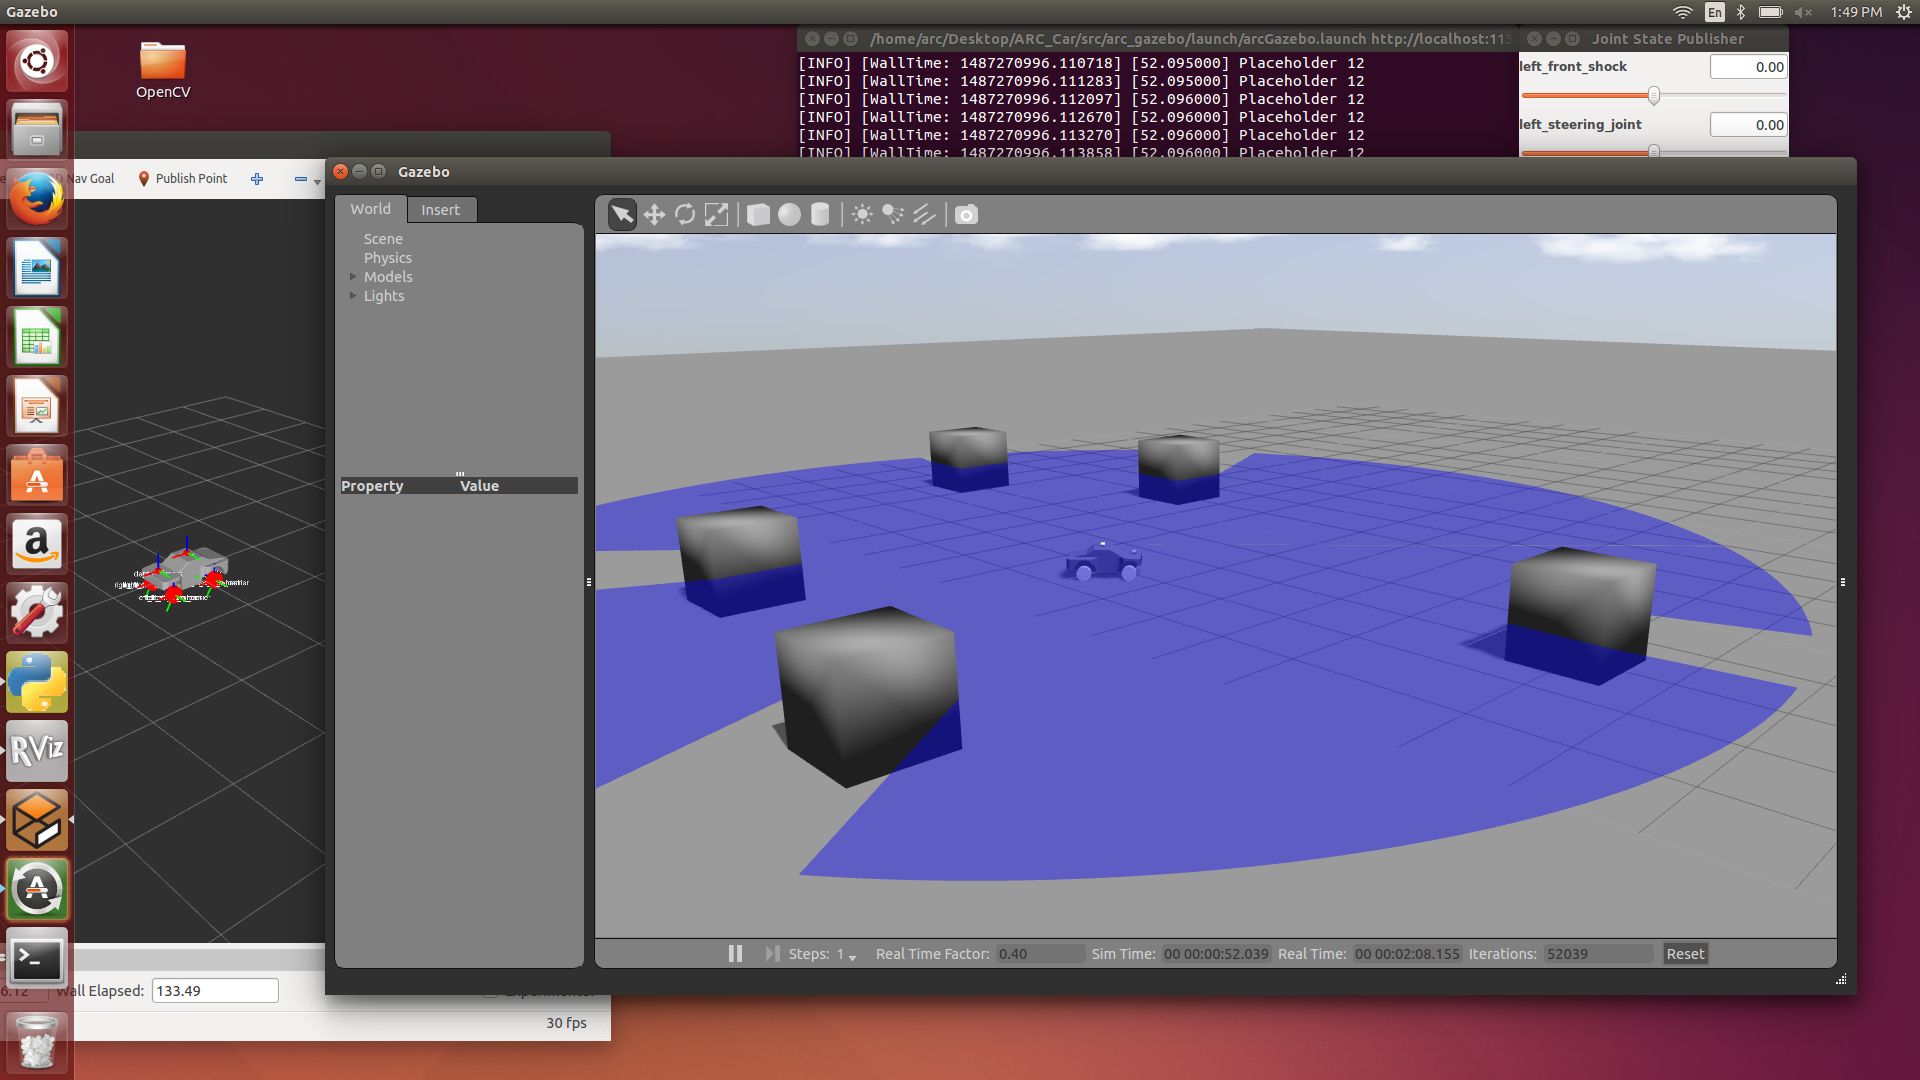
\includegraphics[width=\textwidth]{arc_prog_report_Tao_3}
  \caption{Simulation on a computer}
\end{figure}

My area of focus specified in the design document are: motion model, path planning, and other algorithms. What I am doing right now is related to motion model. I need to get my hands on the actual vehicle to determine the parameters for the motion model. I am not sure if our vehicle uses the Ackerman steering model. If it does, the controller provided by AutoRally is perfect. Otherwise, I will have to assume that our vehicle does use the Ackerman steering model. Luckily, our vehicle is not as big as the one that AutoRally has. The steering model will only have minor effects on the simulation. 

In order to do path planning and experience on other algorithms, I have to have the simulation running first. So I have not started this part yet. Once I have the simulation ready, I will start on the planing algorithms. I will create a publisher that subscribes to data that describes surrounding environment and publishes new waypoints accordingly. This publisher assumes the map of the world is known.

\subsection{Left to do:}
\begin{itemize}
	\item To configure the simulation to accurately simulate our platform, I still edit some parameters in some confiuration and model files. For example, the size and weight of the chassis determine the innertial of the vehicle in the physical engine.  
	\item The two sensors for vision are not working perfectly. They are outputing the right data. However, I can't visualize their outputs on Rviz. I could print out the lidar data on the terminal. I have not try the pointcloud data yet. Rviz keeps complaining that it cannot find the transform frame for the lidar and the camera. Strangly, I was able to visualize the output on Rviz if I used my old model file. I need to double check my model file and the launch files. 
	\item To make the car drive autonomously with minimum obstacle avoidance. Currently, our package does not have the state estimator, the waypoint follower and the constant speed controller, which are all essential for atonomous driving. I need to integrate those components with sensor data to accomplish this task. All of these files resite in the core package, which are hardware specific. Since we are not using any of the hardware that AutoRally uses, I need to potentially take them apart as well. 
\end{itemize}
\subsection{Challenges}
	\begin{itemize}
		\item Time is the issue. There are only 4 weeks left in this term. It is very hard to set a timeline for this project because we don't have a clear view of what is ahead of us. New issues arise constantly. I will try my best to complete the third item on the Left to do list in two weeks.
		\item I will set up the simplist obstacle avoidance procedure at first in the simulation, which is to let the car go from one point to another in a straight line but with a block in between. The vehicle should be able to go around the block to get to its destination. This requires the state estimator to know the current position of the vehicle in a global frame, as well as a waypoint follower to follow pre-defined waypoints. Waypoints are pre-defined point in the global frame. At start, the vehicle should steer towards the first waypoint and then follow the rest. A constant speed controller is also required so that the vehicle can keep its speed even the core software runs in cycles.   
\begin{tabular}{|p{0.3\linewidth}|p{0.3\linewidth}|}
	\hline
	\textbf{Problems} & \textbf{Solutions}\\
	\hline
	Problems that impeded progress. & Specific actions to resolve problems.\\
	\hline
	Visualizing sensor data on Rviz. & Go through all associated files. If it still can't be resolved, I will not use Rviz for visualizing. \\
	\hline
	Getting the car to move without using a controller. & Chase down where the controller commands get sent to. \\
	\hline
	Getting a clear view of the package structure. & I need to start making documentation. \\
	\hline
\end{tabular}

\section{Dan}
\subsection{Current Status}
% what is the current status of your areas of focus?
% Be sure to include descriptions of experimental design and use images, screenshots, code blocks
Much of the work of the first half of the term has been setting up the software environment that will run our RC vehicle.
We have our operating systems installed and configured on our primary computers: the laptop which is the ground control station (GCS), the Raspberry Pi 3 (RPi3) and PXFmini which is the autopilot, and the NUC which is the companion computer that handles the raw calculations. We have ROS installed and running on all platforms.\par

We have been working on getting the RPi3 talking with the PXFMini autopilot cape. The PXFmini autopilot is used to integrate sensor data to send to the NUC and to integrate data coming from the NUC to the vehicle controls. The autopilot also automates calibration of the vehicle and performs other convenient features. We have a system image for the RPi3, from Erle Robotics (the makers of the PXFmini) installed and are able to get the PXFmini launched and armed. This means that the autopilot is ready to take commands.\par
\begin{figure}[H]
	\includegraphics[width=\textwidth]{images/unarmed}
	\caption{PXFmini autopilot before launch and unarmed.}
\end{figure}

\begin{figure}[H]
	\includegraphics[width=\textwidth]{images/armed}
	\caption{PXFmini autopilot after launch and armed.}
\end{figure}

We have also been working on communicating computer-to-computer using ROS nodes. We have run successful tests over direct ethernet connections talking between ROS nodes. These tests lay the groundwork for the NUC to be able to send instructions to the autopilot.\par

While the following areas are all incomplete at this time. However, our accomplishments in each of them pave the way for us to reach the goal of an autonomously controlled RC vehicle.\par

All told, problems with the PXFmini have delayed us from actual hardware testing by about 3 weeks.

\subsubsection{Image Analysis}
No significant progress has been made on image analysis. We still plan to use the ROS rtabmap\_ros package to handle depth-finding and environment mapping. The work Tao has been doing with ROS and Gazebo (a simulation environment) has given our virtual vehicle (running the actual software) the ability to "see" its environment, but we do not have the analysis part of it integrated yet.


\subsubsection{Radio Communication}
\begin{figure}[H]
	\includegraphics[width=\textwidth]{images/radio}
	\caption{3DR Telemetry Radio}
\end{figure}
The status of radio communication is much the same as image analysis. We do not have the physical platform ready for developing and testing radio communication. The radio component of this project should prove to be fairly trivial since radio control and telemetry communication are completely standardized and there are many examples and tutorials, both in hardware and software, to follow. We will be using the MAVLink protocol for radio communication.

\subsubsection{User Interface}
We have a command line interface (CLI) up and running on the GCS, the RPi3, and the NUC. We are using ROS for the CLI. 
Successfully installed ROS on both the GCS and the NUC. This gives us our command line interface (CLI) for issuing commands to the vehicle. We have been using the CLI to send and receive individual commands to ROS topics (a ROS topic is basically the way that ROS sends and receives commands). We are able to publish and subscribe to ROS nodes, specifically MAVros nodes, which is also part of being able to monitor and control the vehicle. We have also run python scripts that have published to ROS topics.\par

\begin{figure}[H]
	\includegraphics[width=\textwidth]{images/imu}
	\caption{Command Line Interface example of a list of running ROS topics.}
\end{figure}



\subsection{Left to do:}
% What do you have left to do?
\subsubsection{Image Analysis}
\begin{itemize}
	\item Integrate data from lidar and cameras into the obstacle avoidance module.
	\item Perform testing and determine if rtabmap\_ros will work for our needs.
\end{itemize}

\subsubsection{Radio Communication}
\begin{itemize}
	\item Connect telemetry radios to the GCS and the NUC.
	\item Create/use ROS topics for reading the telemetry data.
\end{itemize}

\subsubsection{User Interface}
\begin{itemize}
	\item Install and setup a GUI on the GCS for command and control of the vehicle. The most likely candidate at this time is ArduPilot, an open source package that allows fine vehicle control and waypoint selection.
	\item Some of the requirements of the GUI will be:
	\subitem hooking in to telemetry
	\subitem manual override of radio control
	\subitem manual override of autonomous operation
	\subitem ability to set waypoints
	
	\item Fill out CLI functionality. We still need to create custom convenience commands for CLI. Issuing commands to a ROS topic is pretty complicated right now.\par
\end{itemize}

\subsection{Challenges}

\begin{tabular}{|p{0.5\linewidth}|p{0.5\linewidth}|}
	\hline
	\textbf{Problems} & \textbf{Solutions}\\
	\hline	
	Problems that impeded progress. & Specific actions to resolve problems.\\
	\hline
	Did not get RPi3 erle image until late (week 4/5). & Getting the image allowed us to attempt to set up the PXFmini on the RPi3.\\
	\hline
	The first erle image sent was corrupted, it took about a week waiting for a new image. & Erle sent a new image.\\
	\hline
	The environment from Erle seems to be very fragile/unstable. We have run into different problems each time we have re-installed the image they gave us. Our client is have yet a different problem in a separate project where they are trying to use the PXFmini. & This has not been resolved.\\
	\hline
	The PXFmini instructions/tutorials were inconsistent/incorrect. This has created quite a few problems, which has further delayed getting our autopilot running. & We have been working with our client to solve some of the issues with installing and running the PXFmini autopilot.\\
	\hline
	The RPi3 WiFii and ethernet were not configured to connect to the internet. & Researched how to set the RPi3 to connect to the internet via ethernet. It turned out that this problem was caused by how Erle set up their OS image. Found the proper settings to connect to the internet via either WiFi or ethernet. However, if WiFi is set to connect to the internet, external computers cannot talk to the PXFmini via WiFi, same for ethernet.\\
	\hline
	The PXFmini does not respond to commands via MAVros. & MAVros is the ROS api to MAVLink, the protocol for commanding the PXFmini. While we are able to publish (send commands to) and subscribe (get data from) the appropriate topics, the PXFmini does not respond as would be expected. The motors do not activate.\par
	We have found a forum posting stating that a certain variable (SYSID\_MYGCS) needs to be set to 1 in order to override the RC in control to allow computer control of the PXFmini. It looks like the variable can only be set through a GUI, such as ArduPilot. We will try installing ArduPilot on the GCS and see if we can set SYSID\_MYGCS to 1 and see if that makes any difference.\\
	\hline
	My personal laptop died during week 1 & I received a replacement in 2 days and it took another 2-3 days to set my environment back up.\\
	\hline
	Installing Ubuntu 14.04 in dual boot did not go well. It took about a week to get installed properly along side Windows 10. & I wanted a native install of Ubuntu 14.04 (the OS we wanted to use with ROS) on my system to streamline development. Finally got the OS working properly\\
	\hline
	
\end{tabular}

\end{document}
